\section{Penalized Regression} \label{sec:3.PR}
Linear regression is a simple and elegant method for analysing data and constructing models that can be used to make predictions. It is an unbiased estimator and therefor belongs to the class of linear unbiased estimators. Moreover, the theorem of Gauss-Markov~\cite{SIDA2021} tells us that it is the best estimator in its class, which means that its variance is smaller than any other linear unbiased estimator. Unfortunately, there are some problems that arise in certain situations which makes linear regression very bad (i.e. the variance of the coefficients is very high) or even impossible. The solution to these problems give rise to a different class of estimators, called the Bridge estimators~\cite{WWM2020}. This class contains infinitely many estimators, but we will focus on two special cases, called the ridge and Lasso estimators.\\
\\
In this section we will first investigate these problems with linear regression and illustrate them with some code in $R$. Solving these issues will lead us in a very natural way to the ridge and lasso estimators, for which we will also provide illustrations using $R$. We will find that we can fine-tune these estimators further by selecting the right \textit{tuning parameter} $\lambda$. To do this we will need a method to compare different models, which we will address in section~\ref{sec:4.CV&PS}. Finally, we compare the ridge and lasso estimators in section~\ref{sec:5.CRL}.

%----------------------------------------
% --- Linear regression and its flaws ---
%----------------------------------------

\subsection{Linear regression and its flaws} \label{sec:1.1.LR}
Suppose we make observations of $p+1$ variables. Our aim is to predict one of these variables, called the \textit{target}, based on the other $p$ variables, called the \textit{predictors}. If we make $N$ observations, we can construct a \textit{data matrix }
\begin{equation*}
    \textbf{X} = \begin{pmatrix}
    1 & x_{11} & x_{12} & \dots & x_{1p}\\
    1 & x_{21} & x_{22} & \dots & x_{2p}\\
    \vdots & \vdots & \vdots & \ddots & \vdots\\
    1 & x_{N1} & x_{N2} & \dots & x_{Np}
    \end{pmatrix}
\end{equation*}
that contains the predictors of the $i$'th observation in its $i$'th row and  where we added a column of ones in the front. This column of ones will be useful later when we want to calculate the intercept of the regression line. Similarly, we can construct a vector of the targets, called the \textit{target vector}
\begin{equation*}
    \textbf{y} = \begin{pmatrix}
    y_1\\
    y_2\\
    \vdots\\
    y_N
    \end{pmatrix}.
\end{equation*}
The problem now is to find a vector $\beta$ such that $\textbf{X}\beta$ is 'as close as possible' to the target vector \textbf{y}. To this end, we want to minimize the \textit{residual sum of squares (RSS)} defined as
\begin{equation*}
    \textrm{RSS}(\beta) = \sum_{i=1}^N (y_i - \textbf{X}_i \beta)^2
\end{equation*}
where $\textbf{X}_i$ denotes the $i$'th column of $\textbf{X}$, or in matrix notation
\begin{equation*}
    \textrm{RSS}(\beta) = (\textbf{y} - \textbf{X}\beta)^T(\textbf{y} - \textbf{X}\beta).
\end{equation*}
It can be shown~\cite{SIDA2021} that the vector $\hat{\beta}$ that minimizes this expression is
\begin{equation}\label{eq:LSSest}
    \hat{\beta} = (\textbf{X}^T\textbf{X})^{-1}\textbf{X}^T\textbf{y}.
\end{equation}
As mentioned before, the Gauss--Markov theorem tells us that the least squares estimator $\hat{\beta}$ is the one with the smallest variance among all linear unbiased estimators of $\beta$. A first problem with this method of regression is immediately obvious from equation~\ref{eq:LSSest}: What if $\textbf{X}^T\textbf{X}$ is not invertible? This is for example always the case if $p > N$. Furthermore, if $n \approx p$ then the variance of $\hat{\beta}$ will be very large. We illustrate this with a simple example.
\begin{example}
We use the \textit{Hitters} data set of the \textit{ISLR} package in $R$. The code used in this example can be found in \textbf{nog te bepalen}.\\
\\
Firstly, we calculate the regression coefficients using almost all the data available ($250$ observations). The mean squared prediction error can be found in Table~\ref{tab:exampleLSS}. In the next step, we restrict the data we use to the first $100$ observations, apply linear regression on the restricted data and store the mean squared prediction error of the regression parameters in Table~\ref{tab:exampleLSS} below. This process is then repeated for data sets of $75$, $50$, $25$ and $10$ observations.
\begin{table}[ht]
    \centering
    \begin{tabular}{c|c}
         Sample size & Mean Squared Error\\
         \hline
         $250$ & $135825.5$\\
         $100$ & $136102.8$\\
         $75$ & $150103.6$\\
         $50$ & $158626.9$\\
         $25$ & $182158.5$\\
         $10$ & $301629.5$
    \end{tabular}
    \caption{Table of the mean squared errors of some least squares models computed with different amounts of data.}
    \label{tab:exampleLSS}
\end{table}
The general trend of the test errors shown in Table~\ref{tab:exampleLSS} is that they increase as the sample size decreases. If the number of observations gets close to the number of predictors, prediction errors get so large that the model will not be able to accurately predict target values based on observations.\\
\\
One could remark that even when using $250$ data points to compute the model, the test error is still quite large. This can be explained by the nature of the values we are trying to predict. The salary of the baseball players lies mostly in the $400-1000$ range, with some outlier values as low as $<90$ and as high as $>2000$. As a consequence, the variance of the data is high: it takes on the value $204243.4$. Having a mean squared error of $135825.5$ means that, on average, our estimates are about $370$ too low or too high. Given the circumstances, one could argue that this is not too bad.
\end{example}

The reason for the test error in the previous example is that if $n \approx p$, linear regression tends to overfit the data. Even though it is unbiased, little knowledge about the data can be acquired from this model. We say that in these cases, the model has bad \textit{prediction accuracy}. A similar effect can be observed if the predictor variables are (highly) correlated.\\
\\
A second issue with linear regression is that it takes all variables into account. Especially if the number of predictors is high and there is reason to believe some of them may have nothing to do with the target values\footnote{In a medical study, for example, it would be very reasonable to suspect that the predictor "favorite colour" has nothing to do with the target "suffers from heart decease".}, a desired property of regression would be that the coefficients of these 'useless' predictors are zero. This way we can leave them out of the model, thus reducing the complexity of the model, making it easier to understand and interpret.\\
\\
Both of the issues we just laid out have straightforward solutions: in order to reduce overfitting, we could restrict the size of the coefficients by penalizing large values of $\hat{\beta}$ and in order to make the model more interpretable, we could leave out some predictors. Both of these solutions do come at a cost, namely that they introduce some bias into the model. It can be shown, however, that these solutions do lead to a better model as the small sacrifice in bias leads to a giant decrease of variance, increasing the prediction accuracy of the model. This phenomenon is known as the \textit{bias-variance trade-off}.

%----------------------------------
%-------- Ridge regression --------
%----------------------------------

\subsection{Ridge regression} \label{sec:RidgeRegression}
We will work out the ideas at the end of the previous section mathematically. This will lead to what is known as ridge regression.\\
\\
As we already pointed out, we can reduce the overfitting present in regular linear regression by imposing a size constraint on the coefficients. For this we need to be able to measure the \textit{size} of the vector of coefficients $\hat{\beta}$. There are many ways to measure the size of a vector $\textbf{x}$ in mathematics but we will focus on just two of them, namely the $L_1$ and $L_2$ norm, which are defined as follows:
\begin{equation} \label{eq:L1Norm}
    L_1: \hspace{3pt} \norm{\textbf{x}}_1 = \sum_{i=1}^n |x_i|
\end{equation}
\begin{equation} \label{eq:L2Norm}
    L_2: \hspace{3pt} \norm{\textbf{x}}_1 = \sum_{i=1}^n x_i^2
\end{equation}
The $L_1$ norm given in equation~\eqref{eq:L1Norm} will give rise to the Lasso regression, while the $L_2$ norm given in equation~\eqref{eq:L2Norm} will give rise to ridge regression. It is this last one on which we will focus first.\\
\\
The aim is now to calculate
\begin{equation} \label{eq:Ridge}
    \begin{aligned}
        \hat{\beta}{}^{\text{ridge}} = \argmin_{\beta}\bigg\{\sum_{i=1}^N \bigg(y_i - \beta_0 - \sum_{j=1}^p x_{ij}\beta_j\bigg)^2\bigg\} \newline \text{, subject to } \sum_{i=1}^p \beta_i^2 < t
    \end{aligned}
\end{equation}
which is just regular regression, but with the added size constraint on the coefficients. It can be shown that we can rewrite expression~\eqref{eq:Ridge} to
\begin{equation}\label{eq:RidgeAlt}
        \hat{\beta}{}^{\text{ridge}} = \argmin_{\beta}\bigg\{\sum_{i=1}^N \bigg( y_i - \beta_0 - \sum_{j=1}^p x_{ij}\beta_j\bigg)^2 + \lambda \sum_{i=1}^p \beta_i^2\bigg\}
\end{equation}
where $\lambda$ is called the complexity or tuning parameter. The statistician needs to determine the correct value of $\lambda$ to obtain the best model (i.e. the model with the highest prediction accuracy). This can be achieved using a technique called \textit{Cross-Validation}, which we will explain in a later section. It can be shown that the parameter $t$ in equation~\eqref{eq:Ridge} and $\lambda$ in equation~\eqref{eq:RidgeAlt} are in a one-to-one correspondence. Calculating $t$ when $\lambda$ is given is straightforward because $t = \norm{\hat{\beta}{}^{\textrm{ridge}}}^2$. Calculating $\lambda$ for a given $t$ is more difficult. One approach would be to perform ridge regression for a range of values for $\lambda$, then calculate the square of the norm of the regression coefficients and pick the model for which $\norm{\hat{\beta}{}^{\textrm{ridge}}}^2$ is closest to $t$. Another approach could be to start with an initial guess $\lambda_0$, perform ridge regression and calculate $t_0 = \norm{\hat{\beta}{}^{\textrm{ridge}}}^2$. If $t_0 < t$ ($t_0 > t$), choose $\lambda_1 < \lambda_0$ ($\lambda_1 > \lambda_0$) and repeat the process. For this second method we would also need to correctly determine the step length at each step as well as an appropriate error tolerance to ensure the algorithm converges. 

Notice in expressions~\eqref{eq:Ridge} and~\eqref{eq:RidgeAlt} that the penalization term does not involve the intercept $\beta_0$. This is usually a desired property, as penalization of the intercept would make the procedure dependant on the origin chosen for $\textbf{y}$. That is, if we would shift $\textbf{y}$ in some direction by adding a constant $c$ to its components, then this would not simply result in a shift of the predictions by the same amount $c$. We also remark that, like regular regression, ridge regression is sensitive to scale changes. It is therefor advisable to always standardize the data before applying ridge regression.\\
\\
After writing equation~\eqref{eq:RidgeAlt} using matrices $\textbf{X}$, $\textbf{y}$ and $\beta$ as we did in Section~\ref{sec:1.1.LR}, it is not hard to show that
 \begin{equation} \label{eq:ridgeCoef}
    \hat{\beta}{}^{\textrm{ridge}} = (\textbf{X}^T\textbf{X} + \lambda\textbf{I})^{-1}\textbf{X}^T\textbf{y}.
\end{equation}
Important to note here is that the equation above will penalize the intercept if we take our data matrix as we did in Section~\ref{sec:1.1.LR}, namely
\begin{equation*}
    \textbf{X} = \begin{pmatrix}
    1 & x_{11} & x_{12} & \dots & x_{1p}\\
    1 & x_{21} & x_{22} & \dots & x_{2p}\\
    \vdots & \vdots & \vdots & \ddots & \vdots\\
    1 & x_{N1} & x_{N2} & \dots & x_{Np}
    \end{pmatrix}.
\end{equation*}
The column of ones in front is added to calculate the intercept $\beta_0$ automatically, but doing so causes it to be penalized. If this property is not desired, one could opt to not add the column of ones in front of the data matrix, then apply equation~\eqref{eq:ridgeCoef} to get the regression coefficients $\beta_1, \dots, \beta_p$ and calculate the intercept $\beta_0$ separately as, for example, the mean of the target vector.\\
\\
The attentive reader may wonder if the matrix inverse in equation~\eqref{eq:ridgeCoef} always exists. We will prove below that this is indeed the case~\cite{Kj2018}. This means that, contrary to regular regression, we can apply ridge regression in cases where $n < p$.\\
\\
\begin{proof}
    Remark firstly that a matrix of the form $\textbf{X}^T\textbf{X}$ is always positive semidefinite. This can be seen as follows:
    \begin{equation*}
        z^T\textbf{X}^T\textbf{X}z = (\textbf{X}z)^T \textbf{X}z = \norm{\textbf{X}z}_2 \geqslant 0
    \end{equation*}
    The eigenvalues of a positive semidefinite are always bigger than or equal to zero. We show this with a similar argument. Let x be an eigenvalue of a positive semidefinite matrix $\textbf{M}$ with eigenvalue $\gamma$. Then we have:
    \begin{equation*}
        0 \leqslant x^T\textbf{M}x = x^T \gamma x = \gamma \norm{x}_2
    \end{equation*}
    Because $\norm{x}_2 > 0$ if $x \neq 0$ (which is not the case as $x$ is an eigenvector) it follows that $\gamma \geqslant 0$. It is easy to show that if $\gamma$ is an eigenvalue of $\textbf{X}^T\textbf{X}$, then $\gamma + \lambda$ is an eigenvalue of $\textbf{X}^T\textbf{X} + \lambda \textbf{I}$. If $\lambda > 0$, all eigenvalues of $\textbf{X}^T\textbf{X} + \lambda \textbf{I}$ will be strictly positive, so the matrix is invertible.
\end{proof}

% - Theoretical comparison with regular regression -

\subsubsection{Theoretical comparison with regular regression}
To get more insight into formula~\eqref{eq:ridgeCoef}, we compare it to the formula for computing the regular regression coefficients, given in equation~\eqref{eq:LSSest}. For this discussion, we choose to work with the data matrix
\begin{equation*}
    \textbf{X} = \begin{pmatrix}
    x_{11} & x_{12} & \dots & x_{1p}\\
    x_{21} & x_{22} & \dots & x_{2p}\\
    \vdots & \vdots & \ddots & \vdots\\
    x_{N1} & x_{N2} & \dots & x_{Np}
    \end{pmatrix}.
\end{equation*}
and calculate the intercept separately.

We start by computing the singular value decomposition (SVD) of the data-matrix \textbf{X}:
\begin{equation*}
    \textbf{X} = \textbf{UDV}^T.
\end{equation*}
Here $\textbf{U} \in \mathbb{R}^{N \times N}$, $\textbf{D} \in \mathbb{R}^{N \times p}$ and $\textbf{V} \in \mathbb{R}^{p \times p}$. The matrices \textbf{U} and \textbf{V} are orthonormal matrices and the matrix \textbf{D} is a diagonal matrix containing the singular values $d_j$ with $d_1 \geqslant d_2 \geqslant \dots \geqslant d_p$ of \textbf{X}.\\
\\
Substituting \textbf{X} with its SVD in the formula for the regular regression coefficients, we obtain
\begin{align*}
    \textbf{X}\hat{\beta} &  = \textbf{X}(\textbf{X}^T\textbf{X})^{-1}\textbf{X}^T\textbf{y}\\
    & = \textbf{U}\textbf{U}^T\textbf{y}.
\end{align*}
It can be shown~\cite{TB1997} that $\textbf{U}\textbf{U}^T$ is the orthogonal projector onto the column space of \textbf{X}. This gives an important interpretation to linear regression: It calculates the point in the column space of $\textbf{X}$ that is closest to $\textbf{y}$. The coefficients of the linear combination to construct this point from the columns of $\textbf{X}$ are precisely the vector $\hat{\beta}$.

Doing the same for the ridge estimator $\hat{\beta}{}^{\textrm{ridge}}$ we obtain
\begin{align*}
    \textbf{X}\hat{\beta}{}^{\textrm{ridge}} & = \textbf{X}(\textbf{X}^T\textbf{X} + \lambda\textbf{I})^{-1}\textbf{X}^T\textbf{y}\\
    & = \sum_{j=1}^p \textbf{u}_j\frac{d_j^2}{d_j^2 + \lambda}\textbf{u}_j^T\textbf{y}
\end{align*}
We see that, like linear regression, ridge regression computes the coordinates of \textbf{y} with respect to the orthonormal basis \textbf{U}. It then shrinks these coordinates with the factor $\frac{d_j^2}{d_j^2 + \lambda}$. This means that a greater amount of shrinkage is applied to the coordinates of basis vectors that correspond to smaller $d_j$'s. It can be shown that the values $d_j$ also correspond to the principal components of \textbf{X}. The smallest principle component $d_p$ is the one that explains the least amount of variance of the model and gets shrunk the most.

% -- Practical comparison with regular regression -- 

\subsubsection{Practical comparison with regular regression} \label{sec:PractRidgeComparison}
It was previously stated that ridge regression will perform better in situations where data is limited $(n \approx p)$. In this small section, we compare both methods using $R$. We do so using the \textit{Hitters} data set from the $ISLR$ package~\cite{ISL2013}, where we restrict the data to just 4 predictors, namely \textit{Hits}, \textit{Runs}, \textit{Walks} and \textit{Years}, and try to predict the values \textit{Salary}. In order to compare two statistical models, we use \textit{Cross-Validation}. This technique will be explained fully in Section~\ref{sec:4.CV&PS} but we briefly summarize it below:
\begin{center}
    Cross-Validation is a method of assessing the mean squared error (MSE) of a model. The lower the MSE, the better the model.\footnote{It should be noted here that Cross-Validation can be used to measure much more than solely the MSE. Here we choose to use the MSE as it is relatively easy to compute.}
\end{center}

Figure~\ref{fig:RidgeVSLSS} plots the mean squared error of the Ridge model in function of $\log(\lambda)$. The mean squared errors were calculated using Cross-Validation with training sets of size $100$. From the plot it is clear that if we choose $\lambda$ correctly (the value indicated by the blue triangle) we can improve test accuracy if we choose ridge regression over regular least squares.\\
\\
In the literature, ridge (and Lasso) regression are often called \textit{shrinkage methods} as they shrink the regression coefficients towards zero if $\lambda$ increases. This phenomenon is shown in Figure~\ref{fig:CoeffRidge}. 

\begin{figure}
    \centering
    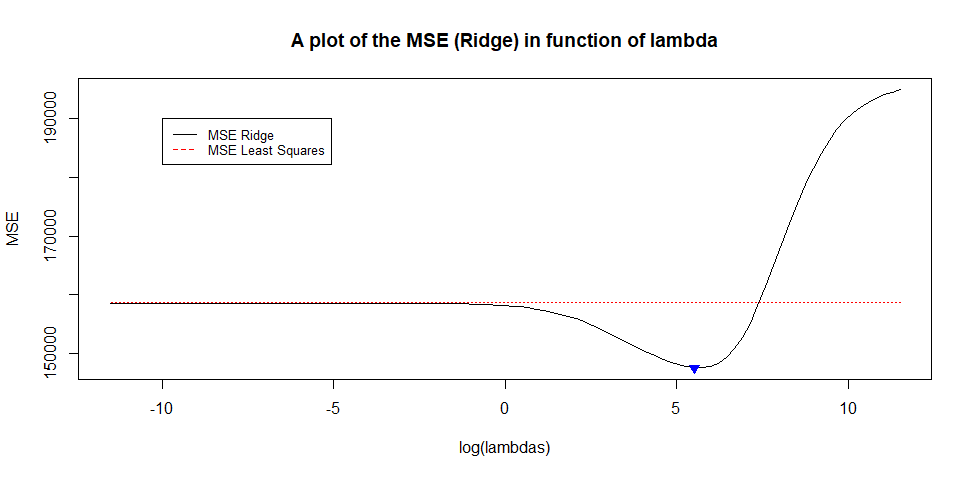
\includegraphics[width=\linewidth]{Figures/RidgeVSLSS.png}
    \caption{A plot of the mean squared error in function of $\lambda$. For reference, the mean squared error of the regular least squares fit is also plotted (red dashed line). The mean squared errors were calculated using Cross-Validation with training sets of size $100$.}
    \label{fig:RidgeVSLSS}
\end{figure}

\begin{figure}
    \centering
    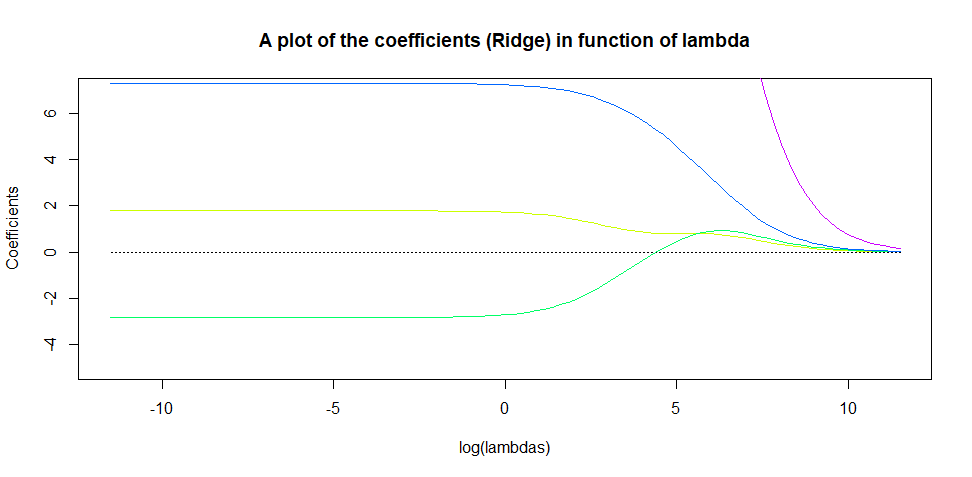
\includegraphics[width=\linewidth]{Figures/CoeffRidgeIFOLambda.png}
    \caption{The size of the regression coefficients plotted in function of $\lambda$.}
    \label{fig:CoeffRidge}
\end{figure}

% -------- A Historical Note ----------

\subsubsection{A Historical note}
The name \textit{ridge} regression was introduced by the inventors Art Hoerl and Bob Kennard. The method finds its origin as a solution to a multivariate optimization problem. The issue Hoerl and Kennard faced was that the optimal/maximal values of there optimization problem all laid on a line, which graphically looks like a ridge of a mountain, hence the name. This made the problem numerically hard to solve, so Hoerl and Kennard had to come up with a better method, which they called \textit{ridge analysis}. This method later found its way into statistics where it is known as \textit{ridge regression}.~\cite{Hoerl2020}

%---------------------------------------
%-------------- the Lasso --------------
%---------------------------------------

\subsection{The Lasso} \label{sec:Lasso}
In the previous section we attempted to solve the issue that regular regression has high variance when $n \approx p$. This led to what is known as ridge regression. There was, however, another problem with regular regression mentioned at the end of Section~\ref{sec:1.1.LR}, namely the issue of model interpretability. While ridge regression shrinks the coefficients towards zero, it does not set any of them equal to zero. The solution to this problem is subtle yet far reaching. It will appear that when we measure the size of the coefficients in $L_1$ norm, the least important coefficients will be set to zero.\\
\\
The Lasso\footnote{The term Lasso is an acronym for 'Least Absolute Shrinkage and Selection Operator'~\cite{Kas2018}} minimizes the following expression:
\begin{equation} \label{eq:Lasso}
    \begin{aligned}
        \hat{\beta}{}^{\text{lasso}} = \argmin_{\beta}\bigg\{\sum_{i=1}^N \bigg(y_i - \beta_0 - \sum_{j=1}^p x_{ij}\beta_j\bigg)^2\bigg\} \newline \text{, subject to } \sum_{i=1}^p |\beta_i| < t.
    \end{aligned}
\end{equation}
Or, equivalently,
\begin{equation}\label{eq:LassoAlt}
    \hat{\beta}{}^{\textrm{lasso}} = \argmin_{\beta}\bigg\{\sum_{i=1}^N \bigg(y_i - \beta_0 - \sum_{j=1}^p x_{ij}\beta_j\bigg)^2 + \lambda \sum_{i=1}^p |\beta_i|\bigg\}.
\end{equation}
Similar to ridge regression, the parameter $\lambda$ should be properly chosen by the statistician. We will explain how in Section~\ref{sec:4.CV&PS}.\\
\\
It is not immediately clear why the Lasso will make some regression coefficients exactly zero. A pictorial representation of the situation, given in Figures~\ref{fig:RidgeContour} and~\ref{fig:LassoContour}, will shed light on this phenomenon. This representation was heavily inspired on Figure 6.7 in \textit{Introduction to Statistical Learning}~\cite{ISL2013}. Figure~\ref{fig:RidgeContour} shows a geometric interpretation of equation~\eqref{eq:RidgeAlt}. We recall this equation below:
\begin{equation*}
    \begin{aligned}
        \hat{\beta}{}^{\text{ridge}} = \argmin_{\beta}\bigg\{\sum_{i=1}^N \bigg(y_i - \beta_0 - \sum_{j=1}^p x_{ij}\beta_j\bigg)^2\bigg\} \newline \text{, subject to } \sum_{i=1}^p \beta_i^2 < t
    \end{aligned}
\end{equation*}
This equation expresses that we want to find the point inside the open sphere $B(0,t)$, where we measure distance using the $L_2$-norm, that minimizes the residual sum of squares (RSS). If we plot the equicontours of the RSS, then the problem can be interpreted as finding the point of intersection of the equicontours with $B(0,t)$. The vector of coefficients obtained using regular regression is shown in the figure as $\hat{\beta}$. If we take $t$ large enough (which corresponds with taking $\lambda$ small enough, i.e. imposing only a small penalty on the size of the regression coefficients), then the blue region will contain $\hat{\beta}$ and the ridge regression coefficients will just be the regular regression coefficients. Building further on this idea we can see that if we set $\lambda = 0$, or equivalently $t = \infty$, ridge regression will always return the regular regression coefficients. This could also be easily seen directly from equation~\eqref{eq:RidgeAlt}.\\
\\
In a completely similar way we can make a geometric interpretation of equation~\eqref{eq:Lasso}. Not only does this aid in getting an intuitive understanding of what the Lasso does, it also shows why the Lasso puts some coefficients equal to zero. The reason for this is that open 'spheres' in $L_1$-norm are squares and thus have corners. Moreover, these corners are located on the axis, which are precisely the points in the coefficient space where some coefficients are equal to zero. It can be seen from Figure~\eqref{fig:LassoContour} that in many cases, the equicontours of the RSS will intersect the blue region in a corner if $\lambda$ is chosen small enough.\\
\\
The extra advantage that the Lasso has over ridge regression does come at a cost: It is more difficult to calculate. The reason for this is that in ridge regression, we want to minimize a quadratic expression with respect to a quadratic constraint. This makes the optimization problem a linear problem, and thus easy to solve. The optimization problem for the Lasso is non-linear due to the non-quadratic constraint. Luckily, there are efficient algorithms available for computing the Lasso just as fast as the ridge coefficients.

\begin{figure}[h!]
    \centering
    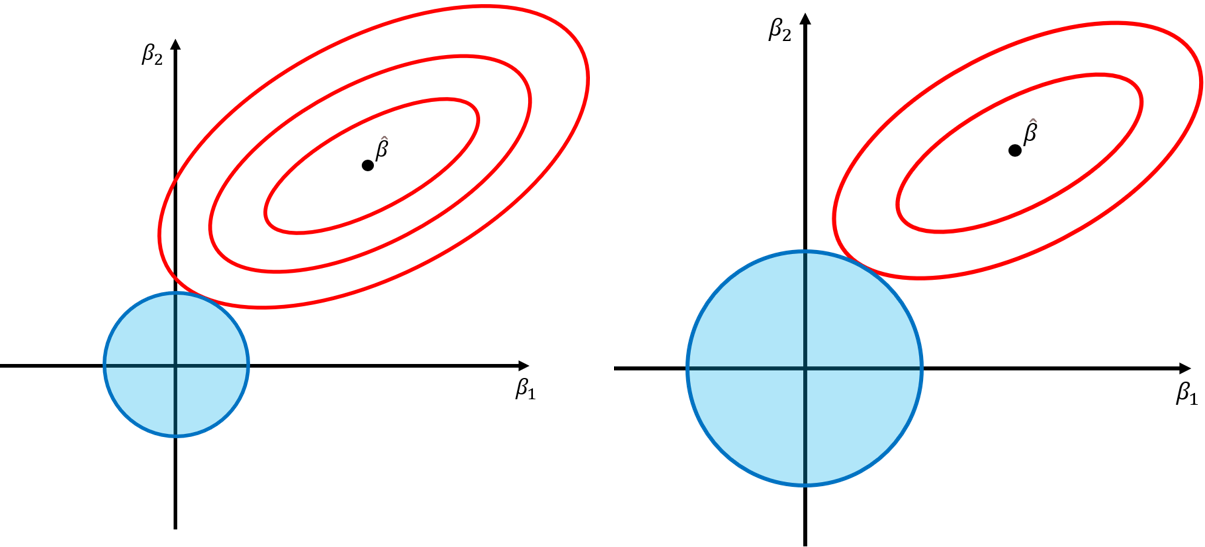
\includegraphics[width = \linewidth]{Figures/RidgeContour.png}
    \caption{The region $L_2(\beta) = \beta_1^2 + \beta_2^2 \leqslant t$ (blue) for two values of $t$ and the equicontours of the residual sum of squares. The point $\hat{\beta}$ represents the regular least squares regression coefficient vector.}
    \label{fig:RidgeContour}
    \vspace{10pt}
    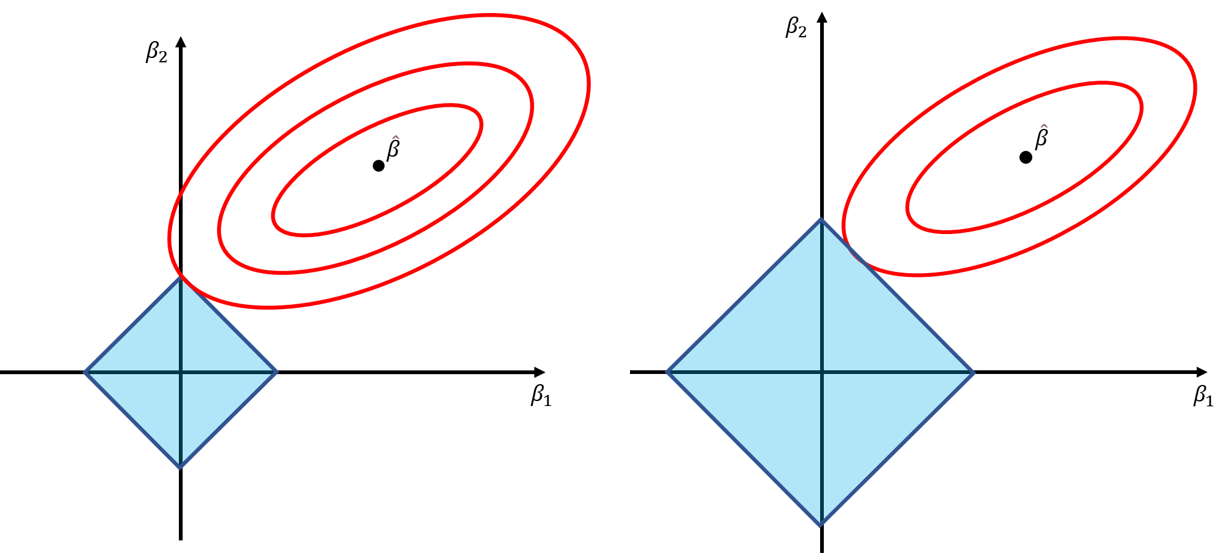
\includegraphics[width = \linewidth]{Figures/LassoContour.png}
    \caption{The region $L_1(\beta) = |\beta_1|+|\beta_2| \leqslant t$ (blue) for two values of $t$ and the equicontours of the residual sum of squares (red). If $t$ is taken small enough, the coefficient $\beta_2$ will be set equal to zero.}
    \label{fig:LassoContour}
\end{figure}

% ------ Comparison with regular regression ---------

\subsubsection{Comparison with regular regression}
In this small section we compare the Lasso to regular regression with an example in $R$ using the same data set as in Section~\ref{sec:PractRidgeComparison} (where we again restrict the data set in the same way). We use Cross-Validation to compute the prediction errors with training sets of size $100$.\\
\\
From Figure~\ref{fig:LassoVSLSS} it is clear that improvement upon the regular least squares fit is possible if we choose the correct value for $\lambda$, indicated by the blue triangle. Note that this is a different value then the one found in Section~\ref{sec:PractRidgeComparison}. As stated in that section, Lasso is a also a shrinkage methods. This is illustrated in Figure~\ref{fig:CoeffLasso}.

\begin{figure}
    \centering
    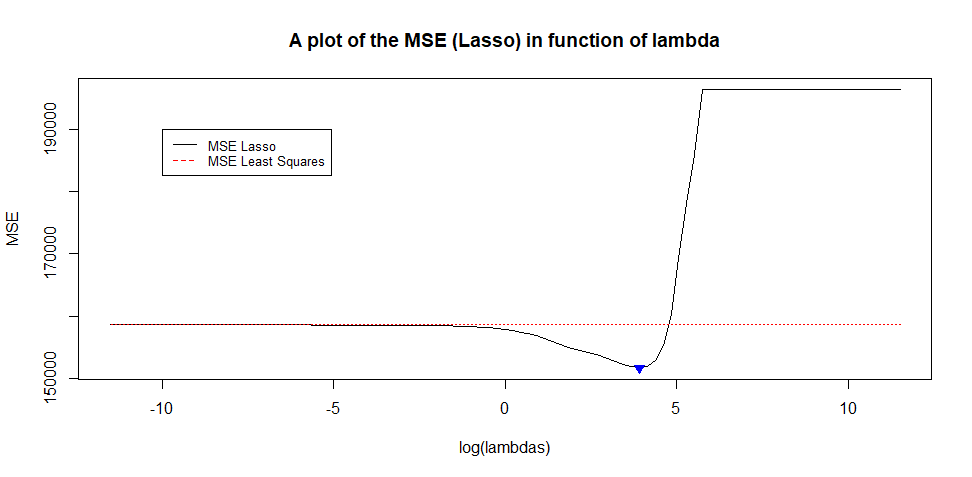
\includegraphics[width=\linewidth]{Figures/LASSOVSLSS.png}
    \caption{A plot of the mean squared error in function of $\lambda$. For reference, the mean squared error of the regular least squares fit is also plotted (red dashed line). The least squared errors were calculated using Cross-Validation with training sets of size $100$.}
    \label{fig:LassoVSLSS}
\end{figure}

\begin{figure}
    \centering
    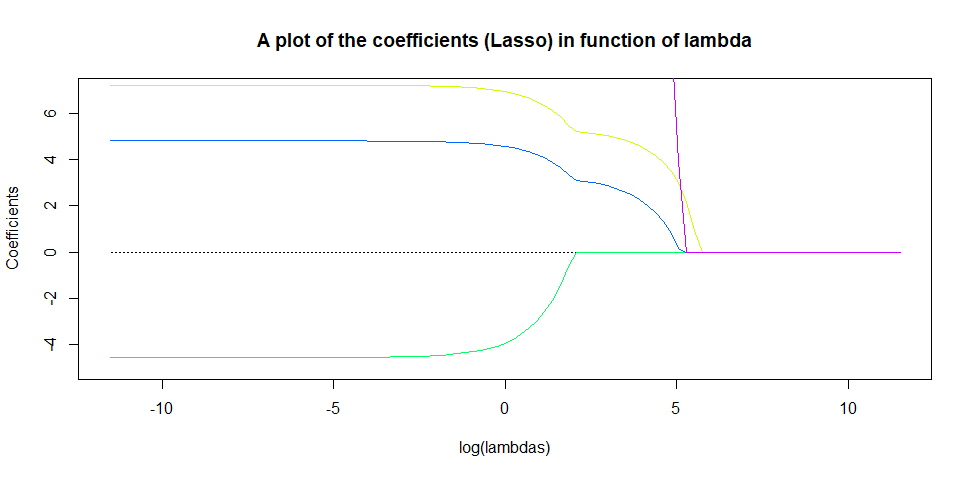
\includegraphics[width = \linewidth]{Figures/CoeffLASSOIFOLambda.png}
    \caption{The coefficients of the Lasso model in function of $\lambda$.}
    \label{fig:CoeffLasso}
\end{figure}

% --------------------------------------------------------
% ---------- Subset selection methods --------------------
% --------------------------------------------------------

\subsection{Subset selection methods}
We conclude this chapter by briefly discussing another approach to improve regular regression. We recall again the two main issues.
\begin{itemize}
    \item \textit{Prediction accuracy}: If $n \gg p$, then least squares fitting will have low variance. However, if $n$ is not much larger than $p$, least squares fitting tends to have high variance (overfitting). If $p > n$, then the variance is even infinite.
    \item \textit{Model interpretability}: Least squares fitting takes all predictors into account. This makes the model often difficult to interpret.
\end{itemize}
In Section~\ref{sec:RidgeRegression} we started by addressing the problem of \textit{prediction accuracy}, which led us to ridge regression. Section~\ref{sec:Lasso} then introduced the Lasso, which also took the issue of \textit{model interpretability} into account. Subset selection methods address the \textit{model interpretability} problem first. They select a subset of the parameters and then perform regular regression on this subset. The difficulty here is in selecting the best subset, that is, the subset for which the model will have the smallest variance.

\subsubsection{Best subset selection}
A naive algorithm to find the best subset is called \textit{Best Subset Selection}. Suppose we want to find the best subset of size $k \leqslant p$. To this end, we can construct all subsets of size $k$ from the set of predictors, calculate for each of these subsets the least squares regression fit and finally, pick the one with the smallest variance. While this is a feasible approach if the number of predictors is not too high $(p \leqslant 40)$\footnote{If $p = 40$ and $k = 20$, we would need to fit a least squares model $\binom{40}{20} \approx 1.4*10^{11}$ times.}, the method quickly becomes computationally too heavy if $p$ increases. Other methods, like \textit{Forward-} of \textit{Backward-stepwise selection} should be used. These methods do not guarantee to select the best subset but require much less computational effort. For further information, we refer to the literature~\cite{ESL2009}~\cite{ISL2013}.